\documentclass{article}
\usepackage[utf8]{inputenc}
\usepackage{geometry}
\usepackage{color}
\usepackage{hyperref}   % use for hypertext links, including those to external documents and URLs
\usepackage{natbib}
\usepackage{graphicx}
\usepackage{float}

\geometry{hmargin=3cm,vmargin=3cm}

\title{\vspace{\fill} Documentation de Validation \vspace{\fill}}

\author{Équipe 17 \\\\ Anaïs Hadj-Azzem - Lucas Grellier - Théo Cachet - Clément Vanhemelryck - César Dumas}

\date{\\}

\hypersetup{
  colorlinks=true,
  linkcolor=blue,
  urlcolor=red,
  linktoc=all
}
% don't need the following. simply use defaults
\setlength{\baselineskip}{16.0pt}    % 16 pt usual spacing between lines

\setlength{\parskip}{3pt plus 2pt}
\setlength{\parindent}{20pt}
\setlength{\oddsidemargin}{1cm}
\setlength{\evensidemargin}{1cm}
\setlength{\marginparsep}{0.75cm}
\setlength{\marginparwidth}{2.5cm}
\setlength{\marginparpush}{1.0cm}
\setlength{\textwidth}{150mm}
\renewcommand{\contentsname}{Table des matières}

\begin{document}

\maketitle
\thispagestyle{empty}
\setcounter{page}{0}
\newpage

\tableofcontents
\thispagestyle{empty}
\setcounter{page}{0}
\newpage

\section{Introduction}

C'est lors de la réalisation d'un projet conséquent que l'on se rend compte du caractère incontournable de la phase de tests. En effet,
nous ne réalisions pas l'impact de cette notion lors des petits projets de l'Ensimag tel que le projet de SGBD, le projet Java ou
bien même le projet C. Ce fut une première pour nous, dans le sens où nous n'avions jamais travaillé à 5 sur un même projet. Dans ce nouvel
environnement de travail, nous avons découvert qu'il faut se mettre d'accord sur des règles et des principes à suivre pour le
bon déroulement du projet. Ce document présente la manière dont notre groupe a appréhendé la phase de validation.
\\\\
Nous commencerons par aborder l'organisation de nos tests et leur contenu dans le détail, puis nous parlerons de notre approche de la gestion des risques.
Nous présenterons aussi dans ce document notre utilisation de l'outil Cobertura et enfin développerons d'autres méthodes de validation
comme celles utilisées pour l'extension ou la relecture de code.

\section{Descriptif des tests}

\subsection{Les différents types de tests}

La quasi totalité de notre base de tests se compose de tests système. Ceux-ci visent à tester l'ensemble du compilateur,
son fonctionnement global, à l’aide de programmes deca. \\
Dans l'ensemble des tests système nous avons deux grandes catégories de tests.
Les tests dit "boîte blanche", qui visent à tester les fonctions en développement, afin de nous assurer qu'elles réalisent bien
ce que l'on attend d'elles. Ensuite nous avons des tests dit "boîte noire", qui ne cherchent pas à tester quelque chose de particulier
dans le code mais qui testent chaque spécification tirée du polycopié Projet GL. \\
Notons qu'un test ne cherche pas toujours à réaliser une fonction valide. On veut parfois intégrer une erreur de manière volontaire pour voir
si notre compilateur y réagi de manière adéquate.
\\
\\
Enfin, nous avons décidé de ne pas nous lancer dans l’écriture de tests unitaires (qui vise à tester une méthode/classe particulière
du compilateur) qui sont bien moins pratique lorsque l'on est en phase
de conception. En effet lorsque l'on développe, nous sommes souvent amenés à modifier nos méthodes et nos classes. Il faudrait alors
ré-écrire ces tests unitaires. Ce qui est, de notre point de vu, trop chronophage.

\subsection{Organisation des tests}
Nous avions dans notre goupe un responsable des tests, qui s'occupait de les homogénéiser et de les valider. Pour permettre une vérification plus rapide de l'exactitude d'un test il a été décidé de mettre en en-tête des
tests une courte description de la fonction testée ainsi que le résultat attendu.\newline
\\
Concernant la structure de notre base de tests, l'arborescence de nos répertoires parle d'elle-même. Nous avons séparé les
tests par partie, puis nous faisons la différence entre les tests censés fonctionner correctement (valides) et les tests davant lever des erreurs à l'exécution (invalides).
\\\\
Dans la partie A ce sont principalement des tests "boîte blanche" qui ont été écris à la suite de l'implémentation du parser et du lexer. Par exemple, on vérifie que tous les caractères du langage deca étaient bien reconnus
 ou à l'inverse que certains caractères n'étaient pas malencontreusement acceptés.
\\
Tandis que dans les parties B et C, à la suite du retour sur le rendu intermédaire,
nous nous sommes rendu compte que les tests "boîte noire" avaient une réelle importance, tout d'abord, car ils permettent de
repérer un maximum de bugs, mais aussi car ils nous aident à mieux comprendre le résultat à atteindre.
Ils nous aident donc à prendre les bonnes décisions lors de la phase ultérieure de codage. \newline
\\
En outre, ce sont les mêmes personnes qui ont implémenté le code et écris les tests : ceci uniquement pour la partie A et B. \newline
Pour la partie C, en complément, des personnes
n'ayant pas participer à la conception du code ont écris de nombreux tests. Lorsqu'un bug était trouvé, la première étape était de trouver à quelle partie du code était liée l'erreur. Puis les personnes les plus à-même
de corriger le bug s'en occupaient en binome ou seul selon la difficulté du bug trouvé. Même lorsque aucun bug n'était trouvé et que la compilation et
l'interprétation par la machine
abstraite réussissaient sans erreur, nous vérifions le code assembleur obtenu pour être sûr que cela correspondait bien à nos attentes et que le résultat obtenu était correct.

\subsection{Les objectifs visés}
\\
Les objectifs des tests étaient multiples. Pour une grande partie, le but était de trouver un maximum de bugs pour pouvoir les corriger : ce sont principalement les tests valides qui jouaient ce rôle.
Un autre objectif était de vérifier que les messages d'erreurs levés correspondaient bien aux attentes de la spécification, notamment pour la partie B, où un grand nombre de tests invalides devant
provoquer des erreurs ont été écris. \newline
Certains tests ont été créés dans le seul but de trouver un potentiel bug sur un point sensible de l'implémentation. A l'inverse beaucoup d'autres avaient pour objectif de couvrir un maximum de situations possibles
sans se focaliser sur une spécificité particulière du compilateur.
\\\\
Enfin, une des finalité importante de ces tests était de pouvoir vérifier que l'implémentation d'une nouvelle fonctionnalité du compilateur ne compromettait pas l'intégrité du reste du code.
C'est pourquoi l'automatisation des tests est un aspect important pour permettre d'effectuer des tests de non-régression du compilateur. Nous développerons cet aspect dans la partie sur les scripts.


\subsection{Les résultats obtenus}
\\
Nous avons une base de test contenant :
\\
\begin{itemize}
\item 87 tests valides et 15 tests invalides pour la partie A
\item 150 tests pour la partie B
\item 70 tests valides, 11 tests invalides et quelques tests interactifs pour la partie C
\end{itemize}
\\
Pour faciliter le lancement de ces tests, nous utilisons des scripts, crées par le responsable des tests de l'équipe.

\section{Les scripts de tests}
\\
Les scripts de tests ont eu un rôle très important pour permettre d'effectuer des tests de non-régression tout au long du projet, permettant ainsi de vérifier au fur et à mesure
du codage que les fonctionnalités déja implémentées n'étaient pas impactées par les nouveautés. Pour cela, nous avons pour chaque étape créer un système de références avec lesquelles les scripts
comparaient les résultats obtenus. Les références étaient créées après vérification par un membre de l'équipe que le résultat était bien celui souhaité.
\\\\
Plusieurs méthodes sont possibles pour lancer les tests en fonction de la fonctionnalité à tester. Pour chaque partie un script permet de lancer le test correspondant(test\_synt, test\_context, decac)
sur la base de test appropriée. Grâce aux oracles présentés précedemment, des tests de non-régression sont facilement exécutables.\newline
Par exemple, en entrant la commande \textit{stage\_b.sh}, doit s'afficher sur le terminal : \newline
\textit{./src/test/deca/context/valid/unprovided/*.deca \newline
Vérification effectuée} \newline
ou bien, dans le cas des tests invalides, c'est à dire censé lever une erreur, le message affiché est : \newline
\textit{./src/test/deca/context/invalid/unprovided/*.deca \newline
Echec attendu de la vérification contextuelle} \newline
Puis, si tout s'est bien déroulé, le dernier message doit être : \newline
\textit{150 tests de vérification contextuelle effectués} \newline
Le principe est identique pour les étapes A et C. Pour la commande \textit{stage\_c.sh}, le résultat
de l'interprétation est aussi affiché pour permettre une vérification en direct du bon résultat du test. \newline
\\
En plus de pouvoir lancer séparemment ces scripts, ils ont été intégrés à l’outil maven.
Il est donc possible à l’aide de la commande \textit{mvn test} (après avoir fait\textit{ mvn test-compile}) de lancer tous les scripts à la suite. Nous vérifions
que tous les tests étaient rangés convenablement et lancions cette commande avant chaque rendu, pour être sur que notre compilateur passait un maximum de test et qu'il n'y avait pas eu régression.
\\\\
Pour finir, certains scripts sont destinés à tester les options tel que celles de vérification ou de décompilation, ou encore
de lancer l'outil de couverture Cobertura sur toute la base de test, et ainsi voir la couverture globale de celle-ci.

\section{Gestion des risques et des rendus}
\\
Suite au rendu intermédiaire de ce 22 janvier dernier, nous avons pu identifier plusieurs risques qui peuvent intervenir dans cette situation,
c’est-à-dire lors d’un rendu client. Pour chacun de ces risques, après discussion et concertation de toute l'équipe nous avons choisi une solution ou une attitude a adopté en conséquence.
Nous avons ensuite agréé que nous suivrions ce qui a été décidé ensemble pour éviter un maximum les conflits et réussir au mieux le projet.
\\\\
Les risques et les solutions sont les suivants :
\\
\begin{itemize}
\item Se rendre compte d’un défaut du rendu quelques minutes avant le rendez-vous le client.\\
\textbf{Solution} : Préalablement, effectuer une grande batterie de tests afin d’éviter toute surprise dans les heures précédant l’heure de rendu. L’utilisation de Cobertura est ici fondamentale.
Plus généralement, éviter les grosses modifications de « dernière minute », qui pourrait causer plus de problème qu’en résoudre, ou si nécessaire créer de nouvelles branches dans le
git afin de pouvoir revenir en arrière rapidement.
\\\\
\item Une erreur est survenue, et le produit rendu au client n’est pas celui voulu.\\
\textbf{Solution} : Avant de rendre le produit au client, un membre de l’équipe récupère le projet entier déposé sur le git, relance une batterie de tests depuis ce rendu, et vérifie le bon fonctionnement de celui-ci.
\\\\
\item Se rendre compte qu’un membre de l’équipe n’a pas effectué le travail prévu.\\
\textbf{Solution} : communiquer tout au long du projet et ne pas hésiter à demander de l’aide à l’équipe.
\\\\
\item Un membre de l’équipe n’est plus disponible, mais personne d’autre n’est formé pour le remplacer.\\
\textbf{Solution}: Pour fournir au client le produit désiré en temps et en heures, il est important que chaque membre de l’équipe prévienne au plus tôt de son indisponibilité, afin que
l’équipe ait le temps nécessaire pour se réorganiser dans les meilleurs délais.
\\\\
\item Le produit rendu n’est pas conforme au cahier des charges\\
\textbf{Solution} : Dans notre cas, relire la spécification et vérifier que tous les fichiers soient placés dans les répertoires demandés. Mais aussi vérifier que les tests sont corrects,
c’est-à-dire qu’ils permettent réellement de tester le bon fonctionnement du produit. Pour cela, un membre est désigné pour la vérification, l’homogénéisation et l’automatisation de tous les tests.
\\\\
\item L’équipe s’est trompée dans la deadline, et le produit n’est pas livrable à la date demandée.\\
\textbf{Solution} : Un membre de l’équipe est chargé de tenir un planning, et de rappeler au reste de l’équipe les deadlines à respecter.
\end{itemize}
\section{Resultats de Cobertura}
\\
Un outil important des étapes de validation et qui a été très utile pour la conception de notre base de test est Cobertura. Cette outil permet en effet de voir quelles lignes du code ont été parcourues(utilisées) par
notre base de test. Cela permet, lorsque l'on le lance sur la base entière de test, de voir quels types de tests n'ont pas encore été écris et sont nécessaires pour détecter un maximum de bugs. Nous avons
tout de même fait attention à ne pas nous appuyer uniquement sur cet outil et à utiliser d'autres méthodes de validation pour notre compilateur.
\\
Voici le résultat de la couverture de notre base de test avec l'outil Cobertura:

\begin{figure}[!h]
  \centering
  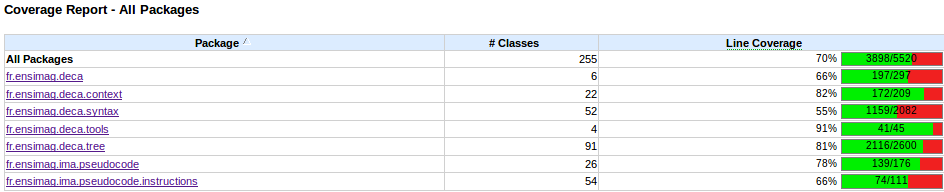
\includegraphics[scale=0.5]{screensCobertura/screenAll1.png}
  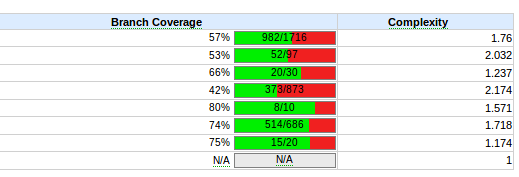
\includegraphics[scale=0.5]{screensCobertura/screenAll2.png}
  \caption{Couverture globale de la base de test}
\end{figure}



\begin{figure}[!h]
  \centering
  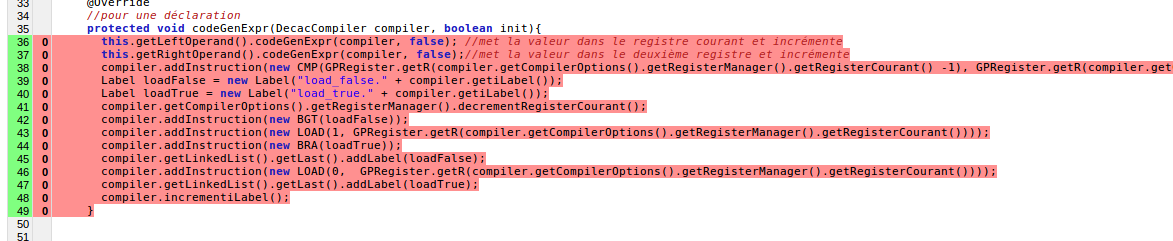
\includegraphics[scale=0.4]{screensCobertura/screenLowerOrEqual.png}
  \caption{Lignes non parcourues de la classe LowerOrEqual}
\end{figure}
\newpage



Le fait que certaines lignes ne soient pas parcourues
peut provenir du fait que certaines fonctionnalités du compilateur aient été testées séparemment. C'est le cas
par exemple, pour les options de decac ou encore pour les readInt et readFloat.
C'est ce que nous pouvons constater sur la figure suivante.(voir figure \ref{optionsCompil}).
\\\\
Mais l’outil reste intéressant, car il nous guide pour l'écriture
de nouveaux tests. Prenons l’exemple du LowerOrEqual dans lequel
nous pouvons remarquer que la fonction codeGenExpr n’a pas été parcouru.Nous décidons alors d’écrire un test pour passer dans cette fonction. C’est un moyen rapide, lorsqu’il est bien utilisé, d’augmenter
la couverture du code de manière ciblée et tester une plus grande partie du compilateur en évitant les répétitions inutiles.

\begin{figure}[!h]
  \centering
  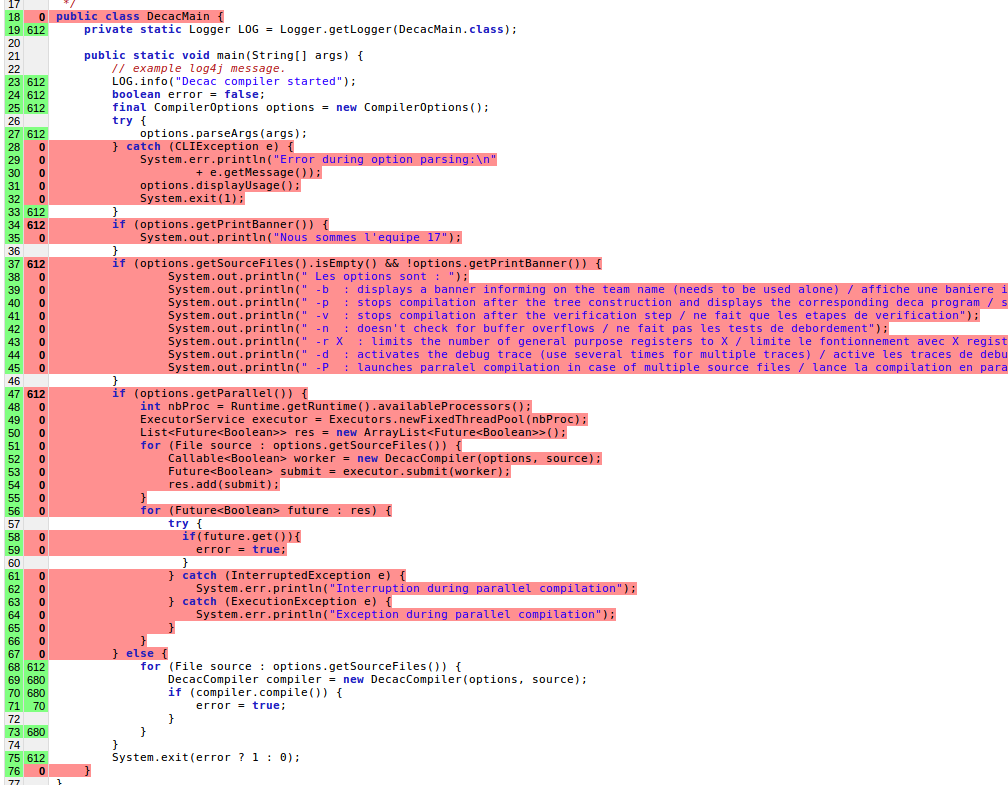
\includegraphics[scale=0.5]{screensCobertura/screenOptions.png}
  \caption{Des lignes des options du compilateur}
  \label{optionsCompil}
\end{figure}

\newpage
Cobertura nous as permis aussi de voir, meme si ce n'est qu'après le rendu, que nous manquions pour la partie génération de code de tests relevant des exceptions au niveau de la compilation.

\begin{figure}[!h]
  \centering
  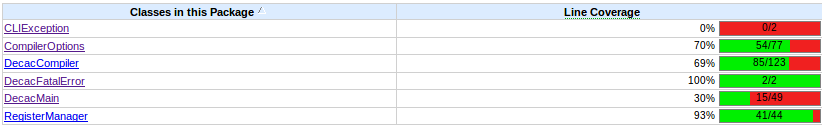
\includegraphics[scale=0.6]{screensCobertura/screenExceptions.png}
  \caption{Des lignes des options du compilateur}
  \label{exceptions}
\end{figure}
\newpage

\section{Méthodes de validation supplémentaires}
\subsection{La classe Math}

\\
La classe Math nous a apporté une aide inattendue concernant le débugage de notre compilateur. En effet, nous pensions que nos 250 tests étaient suffisant
et pouvaient relever toutes les erreurs possibles. Et bien non! Lors de l'intégration de la classe Math, nous avons découvert plus de 10 nouveaux problèmes. Problèmes
pour lesquels nous n'avions donc pas fait de tests (banque de tests à revoir?).\\
C'est donc une grande aide que nous a apporté la classe Math sur ce point. Tous les problèmes trouvés seraient restés inconnus à nos yeux. \\
Pour notre défense nous pouvons dire qu'il est normal de trouver de nouveaux bugs grâce à la classe Math. En effet, il nous semble logique que nous
n'avons pas créé de tests aussi conséquents que l'ensemble de l'extension (500 lignes de code).\\
\\
Nous pouvons, par exemple, citer une partie de l'enrichissement d'arbre qui n'avait pas été traitée dans la partie B. En effet, lorsque l'ont fourni un int à la place
d'un float dans une r-value, il faut que celui-ci soit vu comme un float. Un conv-float est donc nécessaire. Cela a été mis en évidence grâce à l'extension puisque
celle-ci a été développé initialement en Java (donc le responsable de l'extension s'est permis de coder sans faire attention aux règles de grammaire) et qu'elle
 utilise beaucoup d'opérations arithmétiques. C'est une erreur grave, qui nous a permis de remettre en question notre base de tests, que nous pensions jusqu'alors bien complète.
 Nous nous sommes donc remis à écrire plus de tests grâce à Cobertura après cette prise de conscience.
\\
\\ \\
Parlons maintenant des méthodes de validations pour la classe Math et non part la classe Math. En effet, nous avions aussi besoin de tests pour évaluer notre extension et nos
algorithmes. Tester les fonctions trigonométriques avec le terminal seulement ne peut pas être une bonne technique de validation. En effet, la précision de l'extension est variable
suivant l'ensemble de définition des fonctions utilisées. Il n'est donc pas possible d'avoir une idée claire de l'erreur avec les mêmes types de tests que pour le
compilateur Déca.
\\
Nous avons alors décider d'évaluer graphiquement l'extension, afin de pouvoir visualiser et valider efficacement nos algorithmes. Voici par exemple le genre de graphique
que nous obtenons lors de l'évaluation de l'erreur de notre fonction cosinus, dans l'intervalle [-30, 30] avec 100 000 points.\\

\begin{figure}[h!]
    \begin{center}
      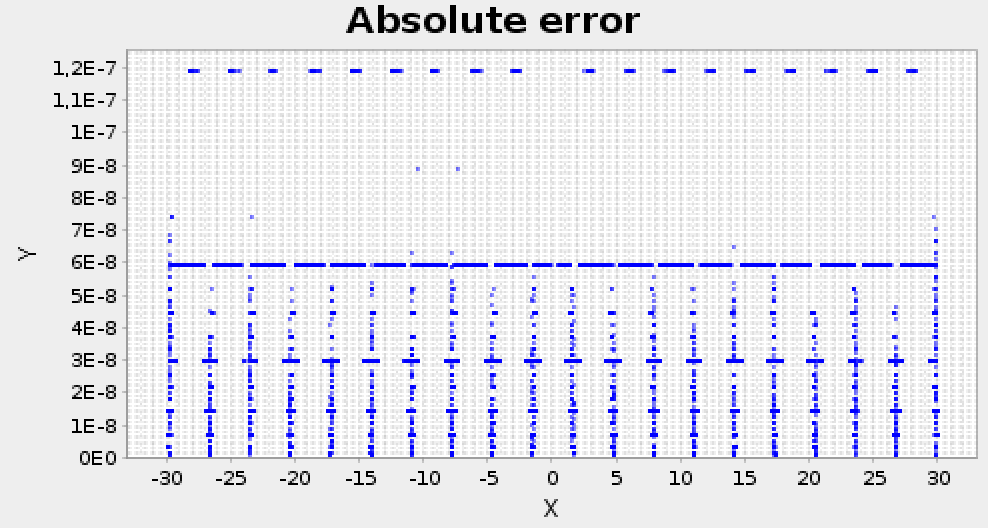
\includegraphics[scale=0.28]{ErrorAbsCosMini.png}
      \caption{Erreur absolue du Cosinus avec 100 000 points}
      \label{Erreur absolue du Cosinus avec 100 000 points}
    \end{center}
\end{figure}


Nous pouvons ici clairement identifier les erreurs, les domaines sur lesquels notre approximation est bonne ou pas. Nottons que nous obtenons une approximation du cosinus
à 0 ou 1 ULP de la valeur de Java dans 94\% des cas (testé et vérifié). Ainsi lorsque nous affichons juste quelques valeurs dans le terminal, nous tombons quasiment tout
le temps sur une valeur exacte et nous pourrions penser alors, à tort, que notre classe Math est parfaite. \\
Ainsi la méthode graphique à une place incontournable dans nos méthodes de validation pour ce projet.

\subsection{La relecture de code}

Une autre méthode de validation utilisée lors de ce projet a été la relecture de code par d'autres membres du groupe. En effet nous travaillions souvent en binôme sur des portions
de code, ce qui permettait de relire le code des autres. Même lorsque nous travaillions seul sur une portion de code bien particulière nous nous faisions un devoir de communiquer
sur la manière d'implémenter choisie pour permettre à un autre membre du groupe de reprendre cette partie si besoin. Notamment dans le cas où un membre du groupe disparaîtrait inopinément, il n'y aurait pas
de parties complétement abandonnée que quelqu'un devrait reprendre du point de départ.
\\
Cette méthode de travail nous as permis aussi lorque quelqu'un était bloqué de recevoir de l'aide sans trop de difficultés puisque nous étions plus ou moins au courant
des différents choix de code pour chaque partie.
Même si bien sur les plus à-même de résoudre les bugs sont ceux qui ont le plus travaillé sur la partie correspondante.
\\
Nous échangions aussi quelques fois avec d'autres groupes lorsque l'on bloquait depuis trop longtemps sur aspect du code ou que nous n'avions pas compris un point précis du polycopié par exemple.

\subsection{Aide du corps professoral}

Dans les méthodes de validation supplémentaires, nous ne pouvons omettre l'aide du corps professoral. Tout au long du sujet, beaucoup de questions se sont soulevées
dans notre groupe. Cela va d'un point un peu flou du polycopié que nous souhaitions éclarcir, à une demande de validation d'une conception. \\
Nous avons par exemple demandé au professeur de valider certaines de nos décisions. Nous avons décidé de faire des tests de type boîte noire, pour tester
chaque règle élémentaire, en amont de la conception. Nous pouvons ainsi voir l'évolution de notre implémentation. L'enseignant nous a alors confirmé que ce choix de
conception était judicieux. Et qu'il nous permettait de surcroît de bien visualiser l'idée derrière chaque règle élémentaire.\\
Nous avions également des questions à propos de l'extension, sur le choix des algorithmes, les manières de procéder ou encore les sources d'information à prioriser.
Une fois encore l'enseignant nous a bien aidé, en mentionnant à titre d'exemple, l'instruction FMA disponible sur la plupart des processeurs récents, qui permet
de n'introduire qu'une erreur machine au lieu de deux dans certaines opérations arithmétiques. Ce qui a eu pour effet de faire progresser l'implémentation actuelle.\\
\\
Bien que nous atteignons la limite du hors sujet, nous tenons à préciser que l'enseignant de SCHEME nous à aussi permis de valider certaines méthodes de travail mises en place et de
corriger les mauvaises. En guise d'exemple, nous n'avions pas donné de rôle bien défini pour chaque membre de l'équipe. Ce conseil nous à alors été procuré lors de la première
séance de suivi. Nous avons alors mis en place cette stratégie et l'équipe fut plus disciplinée et productive.

\section{Conclusion}

Dans ce document, nous avons tenté de vous expliquer, de la manière la plus détaillé possible,
l'organisation et les moyens mis en oeuvre pour mener à bien l'étape essentielle de validation.
Nous retiendrons qu'il y a encoore de nombreuses améliorations à apporter à notre base de tests:
\begin{itemize}
\item Améliorer la couverture. (Regarder précisement les resultats Cobertura et faire des tests spécifiques).
\item Ajouter de nouvelles méthodes de validation que nous n'avons pas mis en place lors de ce projet, mais qui pourrait s'avérer utile
à la conception d'un produit final de meilleur qualité. Par exemple, en vue d'une
base de test toujours plus exhaustive,  il aurait été possible d'utiliser des logiciels pour
écrire des programmes deca aléatoires, même si, bien évidemment,  cette méthode ne serait à utiliser que comme
un complément de la base construite au préalable.
\end{itemize}
\end{document}
